\documentclass{article}

\usepackage{amsmath, amssymb}
\usepackage{tikz}
\usetikzlibrary{automata, arrows.meta, positioning}

\title{1DV517 - Assignment 1}
\author{Xiaoyue Chen}

\begin{document}

\maketitle

\section*{Exercise 1}
\begin{itemize}
	\item \begin{align*}
		      (b+c)^* ((b+c)^* a (b+c)^* a (b+c)^*)^* a (b+c)^* \\
		      + (c^* b^* a c^* b^* a)^* c^* b^*
	      \end{align*}
	\item
	      \begin{align*}
		      (a+b+c)^* a (a+b+c)^* a   \\
		      + (a+b+c)^* b (a+b+c)^* b \\
		      + (a+b+c)^* c (a+b+c)^* c
	      \end{align*}
	\item DFA
	      \begin{figure*}[h!]
		      \centering
		      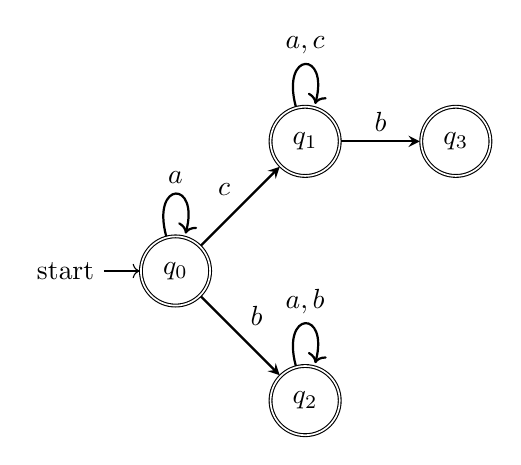
\begin{tikzpicture}[auto]
			      \node (q0) [state, initial, accepting] {$q_0$};
			      \node (q1) [state, above right = of q0, accepting] {$q_1$};
			      \node (q2) [state, below right = of q0, accepting] {$q_2$};
			      \node (q3) [state, right = of q1, accepting] {$q_3$};

			      \path [-stealth, thick]
			      (q0) edge [loop above]
			      node {$a$} ()
			      (q0) edge node {$c$} (q1)
			      (q0) edge node {$b$} (q2)
			      (q1) edge [loop above] node {$a, c$} ()
			      (q1) edge node {$b$} (q3)
			      (q2) edge [loop above] node {$a, b$} ()
			      ;
		      \end{tikzpicture}
	      \end{figure*}
\end{itemize}

\section*{Exercise 2}
$L'$ is regular. Proof:

Since $L$ is regular, $L$ must have an
equivalent NFA. For each transition in this NFA, we remove symbols that are
not in $\Sigma'$. Now, any accepting string defined over
$\Sigma$ is projected over $\Sigma'$ because all
symbols that are not in $\Sigma'$ are removed. The resulting graph
is also an NFA. Hence the new language $L'$ is regular.

\section*{Exercise 3}

\end{document}
